\documentclass[a4paper,11pt]{article}

% Package imports
\usepackage{graphicx}
\usepackage{fancyhdr}
\usepackage{geometry}
\usepackage{titlesec}
\usepackage{wrapfig}
\usepackage{listings}
\usepackage{bm}
\usepackage{chngcntr}
\usepackage{framed}
\usepackage[nolist]{acronym}
\usepackage[most]{tcolorbox}
\usepackage{amsmath, amssymb, amsthm}

\usepackage{needspace} % ensures rule+heading stay together

\newcommand{\rsectionpre}{%
  % Only if not at the top of a page
  \ifdim\pagetotal>0pt
    % If there isn't room for the rule + heading, break first
    \Needspace*{3\baselineskip}%
    % If we didn't break, draw the rule
    \ifdim\pagetotal>0pt
      \noindent\rule{\linewidth}{0.4pt}\par
      \vspace{2em}%
      \nobreak % avoid a break between rule and heading
    \fi
  \fi
}

\titleclass{\rsection}{straight}[\section]

% Tell titlesec how to format \ruledsection
\titleformat{\rsection}[block]
  {\rsectionpre\normalfont\Large\bfseries} % format (rule first)
  {\thesection}{1em}{}

% Optional: starred version \ruledsection* (unnumbered)
\titleformat*{\rsection}{\rsectionpre\normalfont\Large\bfseries}

\titlespacing*{\rsection}
  {0pt}{3.5ex plus 1ex minus .2ex}{2.3ex plus .2ex}

\makeatletter
\let\c@rsection\c@section
\makeatother

% Page layout
\geometry{left=2cm, right=2cm, top=2.5cm, bottom=2.5cm}
\graphicspath{ {./images/} }

% Header definition
\pagestyle{fancy}
\fancyhf{}
\lhead{Introduction to Embedded Systems - WS25/26}
\rhead{\thepage}

% Custom commands for numbered definitions and theorems
\newcounter{definitioncounter}
\newcounter{theoremcounter}
\counterwithin{definitioncounter}{subsection}
\counterwithin{theoremcounter}{subsection}

% Theorem and definition styles with rounded borders and numbering
\newtcolorbox{definitionboxold}{colback=white, colframe=black, arc=5pt, boxrule=1pt, left=5pt, right=5pt, top=5pt, bottom=5pt}
\newtcolorbox{theorembox}{colback=white, colframe=blue, arc=5pt, boxrule=1pt, left=5pt, right=5pt, top=5pt, bottom=5pt}
\newtcolorbox{definitionbar}{
  colback=white,
  enhanced,
  frame hidden,
  borderline west={1pt}{0pt}{black},
  left=6pt,
  top=1pt,
  bottom=1pt
}
\newtcolorbox{definitionbox}[2][]{
  enhanced,
  colback=white,
  colframe=black,
  coltitle=black,
  boxrule=.5pt,
  arc=5pt,
  fonttitle=\bfseries,
%   title filled=true,
  title={Definition \thedefinitioncounter\hspace{.8em}(#2)},
%   title=My Title,
  attach boxed title to top left={yshift=-0.7\baselineskip-0.4pt,xshift=3mm},
  boxed title style={
    colback=white,
    colframe=white,
    left=6pt,
    right=6pt,
    % before upper=\strut
  },
%   boxed title style={tile,size=minimal,left=0.5mm,right=0.5mm, colback=white,before upper=\strut}
  top=10pt,
  bottom=6pt,
  left=6pt,
  right=6pt,
  #1
}
\newtcolorbox{tileddefinitionbox}[2][]{
  enhanced,
  colback=white,
  colframe=black,
  coltitle=black,
  boxrule=.5pt,
  arc=5pt,
  fonttitle=\bfseries,
%   title filled=true,
  title={Definition \thedefinitioncounter\hspace{.8em}(#2)},
%   title=My Title,
  attach boxed title to top left={yshift=-0.7\baselineskip-0.4pt,xshift=3mm},
  boxed title style={
    colback=white,
    colframe=white,
    left=6pt,
    right=6pt,
    % before upper=\strut
  },
%   boxed title style={tile,size=minimal,left=0.5mm,right=0.5mm, colback=white,before upper=\strut}
  top=10pt,
  bottom=6pt,
  left=6pt,
  right=6pt,
  sidebyside,
  sidebyside gap=5mm,
  sidebyside align=center,
  righthand width=0.33\textwidth,
  segmentation hidden,
  #1
}

\setlength{\parindent}{0pt}
\setlength{\skip\footins}{0.5cm} % Adjust this to change the space above the footnotes
\raggedbottom

\newenvironment{leftindent}{\par\leftskip1em\relax\rightskip0cm\relax}
{\par\leftskip0cm\relax\rightskip0cm\relax}

\newcommand{\definition}[2]{%
    \vspace{0.2cm}
    \refstepcounter{definitioncounter}%
    % \textbf{Definition \thedefinitioncounter\hspace{.8em}(#1)}
    % \vspace{0.2cm}\newline
    \begin{definitionbox}{#1}
    #2
    \end{definitionbox}
    % \vspace{0.3cm}
}
\newcommand{\tdefinition}[2]{%
    \vspace{0.2cm}
    \refstepcounter{definitioncounter}%
    % \textbf{Definition \thedefinitioncounter\hspace{.8em}(#1)}
    % \vspace{0.2cm}\newline
    \begin{tileddefinitionbox}{#1}
    #2
    \end{tileddefinitionbox}
    % \vspace{0.3cm}
}

\newcommand{\theorem}[1]{%
    \refstepcounter{theoremcounter}%
    \begin{theorembox}
    \textbf{Theorem \thetheoremcounter:}
    \vspace{0.2cm}\newline
    #1
    \end{theorembox}
    \vspace{0.3cm}
}

\newcommand{\cf}[1]{\[#1\]}
\newcommand{\f}[1]{${#1}$}
\renewcommand{\b}[1]{\textbf{#1}}
\renewcommand{\it}[1]{\textit{#1}}
\newcommand{\pL}{\f{\mathcal{L}}}
\newcommand{\fL}{\mathcal{L}}

\begin{document}

\begin{acronym}[AAAAAA]
    \acro{cps}[CPS]{Cyber-Physical System}
    \acro{es}[ES]{Embedded System}
    \acro{fsm}[FSM]{Finite State Machine}
    \acro{asic}[ASIC]{Application specific integrated circuits}
    \acro{spm}[SPM]{Scratch Pad Memory}
    \acro{dma}[DMA]{Direct Memory Access}
    \acro{irq}[IRQ]{Interrup Request}
\end{acronym}

% Title section
\begin{center}
    {\huge Introduction to Embedded Systems (WS25/26) \par}
    \vspace{0.5cm}
{\large Niklas Rodenbüsch $\quad\mid\quad$ \today \par}
\end{center}
\vspace{0.5cm}


\section{Basics}
\subsection{Terminology \& Definitions}
% \subsubsection{Embedded Systems}
\definition{Embedded Systems}{\ac{es} are information processing systems embedded into a larger (technical) product, controlling the larger system or providing information processing for it.}

\definition{Embedded Software}{Embedded software is computer software, written to control embedded systems. Typically specialized for the particular hardware that it runs on and has time and memory constraints.}

\definition{\ac{cps}}{Complex network of \b{real-time} interacting elements (e.g. \ac{es}) with physical input and output instead of standalone devices.}

\subsection{Applications}
\ac{es} can be applied to a multitude of different domains, such as:
\begin{itemize}
    \item \b{Automotives:} ABS, ESP, Airbags, \dots
    \item \b{Aerospace:} Anti-Collision, Flap control, \dots
    \item \b{Wearables:} Glasses, Watches, ...
\end{itemize}

\subsection{Characteristics}
\ac{es} must be any number of the below characteristics (depending on the requirements, \b{not} all at once):
\begin{enumerate}
    \item \b{Efficiency:} Energy, Area (Hardware), Code-size, Run-time, Weight, Cost
    \item \b{Dependable:} Reliability \f{P}(system working correctly after working at \f{t=0}); Maintainability \f{P}(system working correctly \f{t} time steps after error); Availability \f{P}(system working at \f{t}); Safety; Security (confidential data \& authentic communication)
    \item \b{Real-Time cabable:} System must react to stimuli within a given time interval; late reactions arriving too late are wrong; hard-constrained = if failure to meet the constraint results in catastrophe (else soft-constrained); response has to be guaranteed without statistical arguments
    \item \b{Reactivity:} Superset of real-time constraint; behaviour of system depends on input and current state (can be modeled as automata); continuous interaction with environment (at a pace given by the environment) through sensors and actuators
\end{enumerate}

\subsection{Components / Feedback loop}
The feedback loop typically contains: (1) Sensor(s), (2) Information Processing Unit, (3) Actuator(s), (4) Memory and the
(5) Environment. Depending on the ES some of them are optional or simply not needed. Example below: battery charging system.

\vspace{0.5cm}
\begin{figure}[h!]
    \centering
    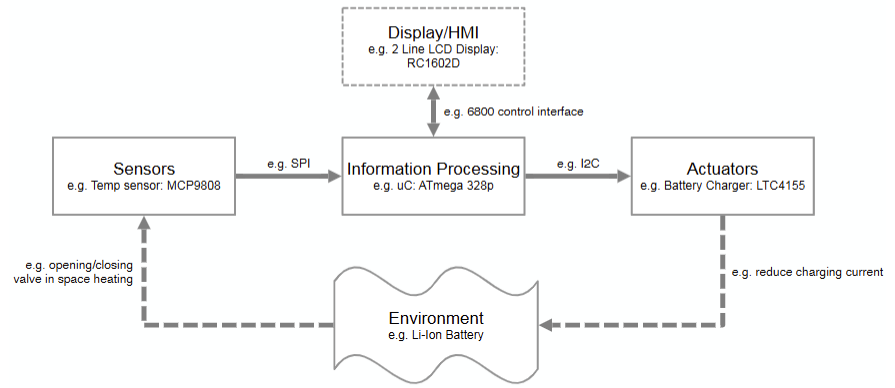
\includegraphics[width=0.8\textwidth]{1_components.png}
\end{figure}
\section{Specification}
The first step of designing an \ac{es} is to translate the description into a formal specification, and \b{prove} that the specs meet the goals the system.
\subsection{Abstraction/Hierarchy}
\begin{itemize}
    \item \b{Behavioural hierarchy:} Describe the systems overall behaviour (states, events, outputs)
    \item \b{Structural hierarchy:} Describe the physical composition (processors, actuators, sensors)
\end{itemize}
\subsection{Timing Behaviour}
Since \ac{es} are real-time systems, explicit timing requirements must be specified: \\[0.5em]
\b{(1)} Elapsed time for execution; \b{(2)} Delay of processes; \b{(3)} Timeouts for events; \\
\b{(4)} Deadlines for task finishing
\subsection{Dependable Systems}
Dependable systems fulfill the following requirements: \\[0.5em]
\b{(1)} Unambiguous semantics; \b{(2)} Support formal verification; \b{(3)} Are executable; \\
\b{(4)} Appropriate model for computation (execution model for each component, communication model)
\subsection{Further Specifications}
\begin{itemize}
    \item \b{Event-Handling:} Specify how internal \& external events are handled.
    \item \b{Concurrency:} Specify how distributed and parallel operations happen.
    \item \b{Synchronization and Communication:} Communication (i.e. mutual exclusion) between components
    \item \b{Non-functional properties:} Fault tolerance, Weight, Size, Power consumption, ...
\end{itemize}
\subsection{Computational Specifications}
\begin{itemize}
    \item \b{Presence of programming elements} (i.e. arithmetic operations, loops, function calls)
    \item \b{Executability:} Plausibility checking
    \item \b{Readability}
    \item \b{Domain-Specific support}
\end{itemize}











\section{\ac{fsm}}
An FSM is a (graphical exception-oriented) model for the internal state of an embedded system (desribes states, actions and how to handle exceptions). Inputs are internal/external events, and states are the memory content after events.\\ 
FSM can be used for e.g. input validation, concurrent event handling, or program flow (interrupt handling).
\tdefinition{FSM / Acceptor}{
    \f{M = (I, S, s_0, \delta, F)} is a deterministic finite automataton, iff:
        \begin{itemize}
            \item \f{I} is a finite, non-empty set of input symbols
            \item \f{S} is a finite, non-empty set of states
            \item \f{s_0 \in S} is the initial state
            \item \f{\delta: S\times I \rightarrow S} as transition function
            \item \f{F\subseteq S} are final (accepted) states
        \end{itemize}

    \tcblower

    \centering
    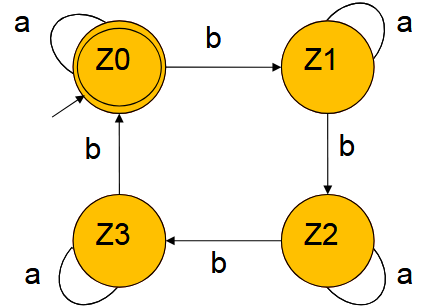
\includegraphics[width=.9\linewidth]{fsm.png}
}
\subsection{Moore and Mealy Machines}
\tdefinition{Moore Machine}{
    Moore machines \f{(I, O, S, s_0, \delta, F, \lambda)} extend acceptors by:
    \begin{itemize}
        \item \f{O} as a finite, non-empty set of output symbols
        \item \f{\lambda: S\rightarrow O} as output function
    \end{itemize}
    The Moore Machine on the right outputs the result of \f{c\%4}.\\
    Note: For an input of length \f{n}, we get \f{n+1} outputs, as we get to \f{s_0} using the empty input symbol \f{w_0 = \epsilon}.
    % \vspace*{0.5cm}
    \tcblower

    \centering
    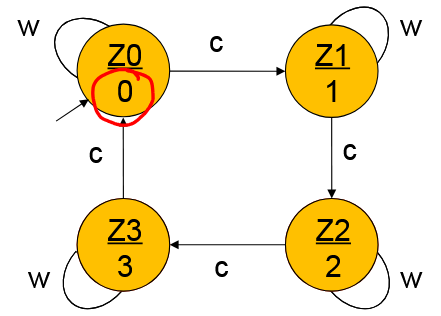
\includegraphics[width=.8\linewidth]{moore.png}
}
\tdefinition{Mealy Machine}{
    Mealy machines \f{(I, O, S, s_0, \delta, F, \lambda)} differ from Moore machines in their output function: \f{\lambda: S\times I \rightarrow O}\\
    Mealy machines create outputs during state transitions, with the output for the initial transition being '-'.\\

    Examples: Enigma, Traffic light, Number classification, ...
    \tcblower
    \centering
    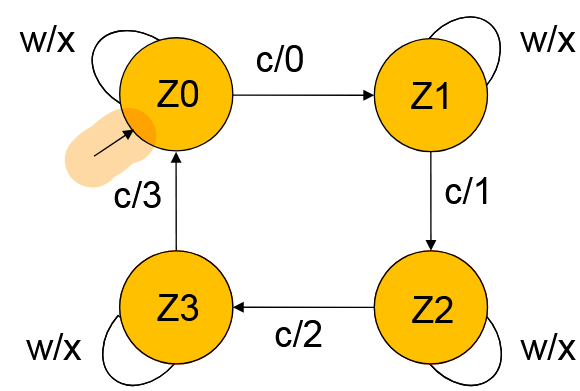
\includegraphics[width=.8\linewidth]{mealy.png}
}

Mealy machines depend on the current state and the current input symbol, while Moore machines can be seen as special Mealy machines where the output does not depend on the current input symbol.\\[0.5em]
\b{Important:} Moore can be transformed into Mealy and (partially) vice versa.

\section{Statecharts}
Especially when dealing with complex systems (many states) and/or concurrency, Moore and Mealy are not useful. Statecharts extend the classical machines with concepts like non-determinism (OR), history, variables, concurrency (AND), and timing/simulation.\\[0.5em]
Statecharts produce I/O differently as well: Transitions can be active on the presence of events, produce events, or change variables.\\[0.5em]
\b{Real-world examples:} Automotive applications (industry standard), UML

\subsection{Transitions}
% \begin{wrapfigure}{R}{.3\textwidth}
%     \centering
%     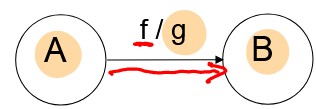
\includegraphics[width=.9\linewidth]{sc1.png}
% \end{wrapfigure}
A transition from state A to B occurs iff event f is present while being in A. On transition the event \f{g} is produced. Produced events exist for one step only.
\begin{figure}[h]
    \centering
    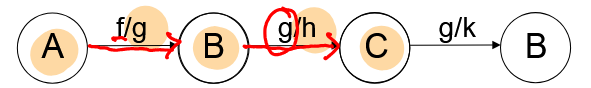
\includegraphics[width=.5\textwidth]{cs2.png}
\end{figure}

\subsection{Non-Determinism}
Multiple events can be present at the same time. While non-deterministic transitions are possible, tools usually warn beforehand so they can be handled using e.g. priority specification (see below).

\subsection{Hierarchy}
Statecharts introduce superstates \f{S}. Superstates S are called \b{OR}-superstates, if exactly one of the substates of \f{S} is active whenever \f{S} is active.\\
\begin{figure}[h]
    \centering
    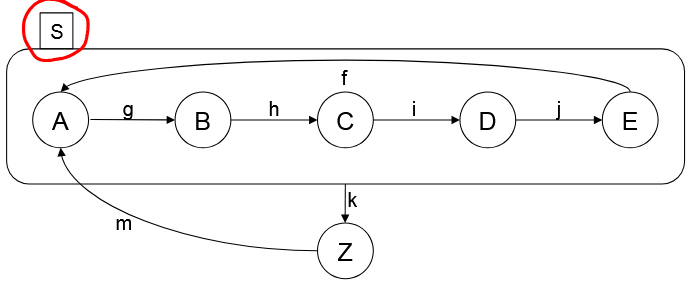
\includegraphics[width=.5\textwidth]{sc3.png}
\end{figure}

Current states of statecharts are called active states. States that are not composed of other states are called basic states. States containing other states are called superstates. For each basic state s, the superstates containing s are called ancestor states. When a basic state is active, all its ancestor states are active too.\\
The state hiearchy can be represented as a tree, where basic states are the leafs. The highest level in the hierarchy has priority when multiple transitions (i.e. events) are active at the same time.

\subsection{History}
To determine which substate is entered when a superstate is entered, different history mechanisms can be used. \b{Note:} Nested superstates need a default state each!
\begin{itemize}
    \item \b{Default:} Filled circle (not a state itself) pointing to a substate. Entered each time \f{S} is entered.
    \item \b{History:} Enters substate \f{S} was in before \f{S} was left, or default if \f{S} entered for the first time.
    \item \b{Deep History:} Deep history remembers states at the sub-hierarchy level too!
\end{itemize}

\subsection{Event-Condition-Action}
Statecharts include typed variables (e.g. numbers) to represent data (states + variables = \it{status}). Values of variables keep their value until they are reassigned. Values of variables are visible to all parts of a statechart (shared memory). New values become effective in the execution stage for the current step and are obtained by all parts of the model in the \it{following} step.\\[0.5em]
This makes transition functions possible: A transition may be taken if an event occured in the last step AND a condition referring to a variable is true. Actions can then either be variable assignments or creation of events.\\

\b{Event types:} Atomic events (A, B, BUTTON), entering/exciting state \f{en(S)/ex(S)}, variable value change \f{ch(x)}, access to variable \f{rd(x)/wr(x)}, condition value changes \f{tr(co)/fs(co)}\\

\b{Condition types:} Atomic conditions, constants (true/false), relations between values, residing in a state \f{in(S)}\\

\b{Action types:} Atomic actions, emmitting events \f{raise(E)}, variable assignment, compound actions, list of actions, conditional actions

\subsection{Concurrency}
Concurrency can be expressed via \b{AND}-Superstates, where \it{all} substates are active when \f{S} is active.\\[0.5em]
\b{Important}: Concurrency can lead to different types of conflicts (e.g. write-write if two parallel transitions write the same variable). 

\subsection{Timers}
Statecharts support special timeout events, e.g. "if event \f{a} does not happen while being in state \f{X} for 20ms, a timout event will take place and activate state \f{Y}".

\subsection{Simulation}
Execution of a statechart consists of a sequence of steps (arbitrarily small time), each leading from one \it{status} to another. At each step, the current system status \f{s_i}, the current time \f{t}, and internal/external changes \f{\Delta} are given. The goal then is to find the internal events \f{e_i} and new status \f{s_{i+1}}.\\
External events not yet seen in the previous step and changes of external data not seen in the previous step are called external changes for the current step.\\[0.5em]
\b{Status} now consists of: active states, values of variables, generated events from previous steps, values of history connectors, set of all timeout events.

\subsubsection{Simulation Step}
(1) Update timeout events \f{\ \rightarrow\ } (2) Determine sequence of transitions to be taken, based on current i/e events and i/e variables \f{\ \rightarrow\ } (3) Compute next states and actions \f{\ \rightarrow\ } (4) Apply transitions

\subsection{Pros and Cons}
\begin{table}[h!]
\begin{tabular}{|p{.45\textwidth}|p{.475\textwidth}|}\hline
\textbf{Andvantages}                                          & \textbf{Disadvantages}                           \\\hline\hline
Simple transformation into hard- and software implementations & Complex for large systems                        \\\hline
Efficient for simulation                                      & Not useful for distributed applications          \\\hline
Basis for formal verification                                 & No formal representations of operations and data \\\hline
Arbitrary nesting of superstates possible                     & Large part of status is hidden in variables      \\\hline
\end{tabular}
\end{table}









\section{Petri/CE/PT Nets}
In contrast to hierarchical state machines, state transitions in Petri Nets are asynchronous. Focus on modelling causal dependencies; no global synchronization assumed \f{\ \rightarrow\ } message passing only. Petri nets can be used to model concurrent distributed systems (e.g. UML).
\begin{figure}[h!]
    \centering
    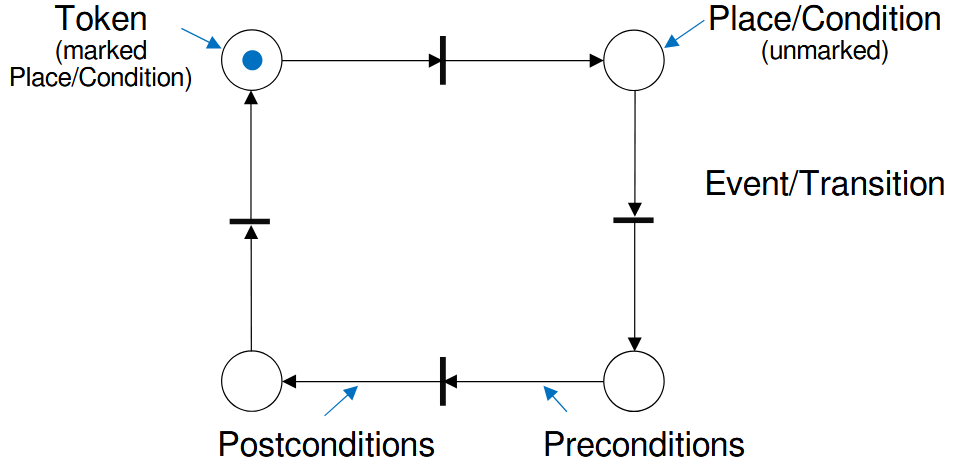
\includegraphics[width=.5\textwidth]{petri.png}
\end{figure}

\subsection{Components}
\begin{itemize}
    \item \b{Conditions:} Represent "local states" and are either met or not met (potential state space)
    \item \b{Events:} May take place if certain conditions are met (represents state transition)
    \item \b{Flow relation:} Relates conditions and events
    \item \b{Tokens:} Assignment of tokens to conditions specify a global state 
\end{itemize}
\definition{Petri Net}{
    A Petri Net \f{N = (C,E,F,M_0)} is defined with:
    \begin{enumerate}
        \item \f{C}: set of conditions/places
        \item \f{E}: set of events/transitions
        \item \f{F}: set of edges (binary flow relations) with \f{F\subseteq(C\times E)\cup(E\times C),\quad}\f{C} and \f{E} disjoint
        \item \f{M_0: C\rightarrow \mathbb{N}} as the initial marking
    \end{enumerate}
} 
\definition{Preconditions / Postconditions}{
    Let \f{N} be a Petri Net and let \f{x\in E, y\in C}:
    \begin{enumerate}
        \item \f{\cdot x := \left\{y\ |\ (y\times x)\in F\right\}} is called the set of preconditions
        \item \f{x\cdot := \left\{y\ |\ (x\times y)\in F\right\}} is called the set of postconditions
    \end{enumerate}
}

\subsection{Marking}
A marking is a mapping \f{M:C\rightarrow\left\{0,1\right\}}. Firing event \f{x} generates new markings on all conditions \f{C} according to the following rules:
\begin{enumerate}
    \item An event \f{x} can be fired, iff \f{\cdot x} is marked and \f{x\cdot} is unmarked
    \item After firing, \f{\cdot x} is unmarked and \f{x\cdot} is marked
    \item \f{M\rightarrow M'}, iff \f{M'} results from \f{M} by firing \it{exactly} one transition
\end{enumerate}

\subsection{Condition-Event Nets}
\definition{Different Concepts}{
    \begin{enumerate}
        \item \f{(c,e)\in C\times E\rightarrow (c,e)} is called \b{loop} iff \f{cFe\wedge eFc}.
        \item Net \f{N=(C,E,F)} is called \b{pure}, if \f{F} does not contain loops.
        \item Net is called \b{simple}, if there are no two transitions that have the same sets of input and output places: \f{\forall x,y\in E: \cdot x = \cdot y \wedge x\cdot = y\cdot \ \Rightarrow\  x=y}
    \end{enumerate}
}
\definition{C/E-Nets}{
    A Petri Net \f{N=(C,E,F)} together with a non-empty set of markings \f{M} is called C/E-Net, iff:
    \begin{itemize}
        \item \f{N} is simple, pure, ad has no isolated elements
        \item \f{M} is closed wrt. "firing" and "inverse firing"
        \item \f{N} is deadlock-free: For each event \f{e\in E} exists a marking \f{m\in M} that allows firing at \f{e}
    \end{itemize}
}
\subsection{Properties}
\begin{itemize}
    \item Marking \f{M'} is \b{reachable} from marking \f{M}, iff there exists a sequence of firings that transform \f{M} into \f{M'}
    \item C/E net is \b{cyclic}, iff any two markings are reachable from each other
    \item C/E net fulfills \b{liveness}, iff \f{N} is deadlock-free
    \begin{itemize}
        \item \b{Strong liveness:} For each \f{M} and \f{e} exists \f{M'} so that \f{M'} is reachable from \f{M} and \f{M'} activates \f{e} for firing.
        \item \b{Weak liveness:} For each \f{M} an event \f{e} exists so that \f{M} activates \f{e} for firing.
    \end{itemize}
\end{itemize}

\subsection{Place/Transition Nets}
PT-Nets can model resource (i.e. producer/consumer) usage and causal relationships, by allowing more than one token per condition, capacities of places, and weights of edges. The downside is that the state space may become infinite.\\
Nets can be used to verifiy properties such as reachability, liveness, or bounds on the number of tokens.

\definition{PT-Nets}{
    A net \f{N=(P,T,F,K,W,M_0)} is called PT-Net (non-deterministic), iff:
    \begin{itemize}
        \item \f{N=(P,T,F)} is a net with places \f{p\in P} and transitions \f{t\in T}
        \item \f{K:P\rightarrow (N_0\cup\left\{\omega\right\})\backslash \left\{0\right\}} denotes the capacity of places; \f{\omega\equiv \infty} capacity. A place \f{p_i} can hold \f{K(p_i)} tokens at maximum.
        \item \f{W: F\rightarrow (N_0\backslash \left\{0\right\})} denotes the weight of graph edges
        \item \f{M_0: P\rightarrow N_0\cup\left\{\omega\right\}} represents the initial marking of places
    \end{itemize}
    A net \f{N} is \b{contact-free}, if capacities in \f{\cdot t} never prevent activation of the transition \f{t}. A \b{pure} and \b{contact-free} PT-Net is completely defined by \f{N} and \f{M_0}.\\
    Since capacities of places are not considered in \f{N} (here: matrix \f{P\times T}), we can not always compute transitions!
}
\begin{figure}[h!]
    \centering
    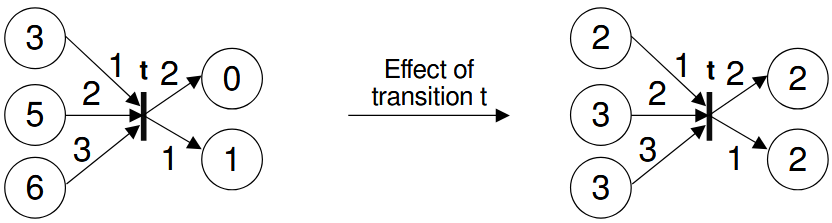
\includegraphics[width=.7\textwidth]{ptnet.png}
\end{figure}

\subsubsection{Pros and Cons}
\begin{table}[h!]
\begin{tabular}{|p{.45\textwidth}|p{.475\textwidth}|}\hline
\textbf{Andvantages}                                          & \textbf{Disadvantages}                           \\\hline\hline
Can model distributed applications & problems with modeling timing \\\hline
Well-known theory for proving properties & no programming elements \\\hline
                                 & no hierarchy \\\hline
\end{tabular}
\end{table}











\section{Design Space Exploration and Optimization}
The design space of ES has many different parameters and aspects that can be optimized, thus yielding a multiobjective optimisation problem. Examples are:\\[0.5em]
\b{Design Space:} Cost, Performance, Energy, Quality, \dots\\[.5em]
\b{Implementation:} \acp{asic}, memory architectures, interfaces (I$^2$C, SPI, CAN), Sensors \& Actuators, programmable devices (microcontrollers/-processors), ...\\[.5em]
\b{Processing:} Clock frequency, OPS, Bandwidth, FPS, Worst-Case vs. Average-Case performance, ...\\[0.5em]
Individual elements of the design space can be further split up into multiple aspects, e.g. cost \f{\rightarrow} manufacturing cost, design cost, administration, ...
\begin{figure}[th!]
    \centering
    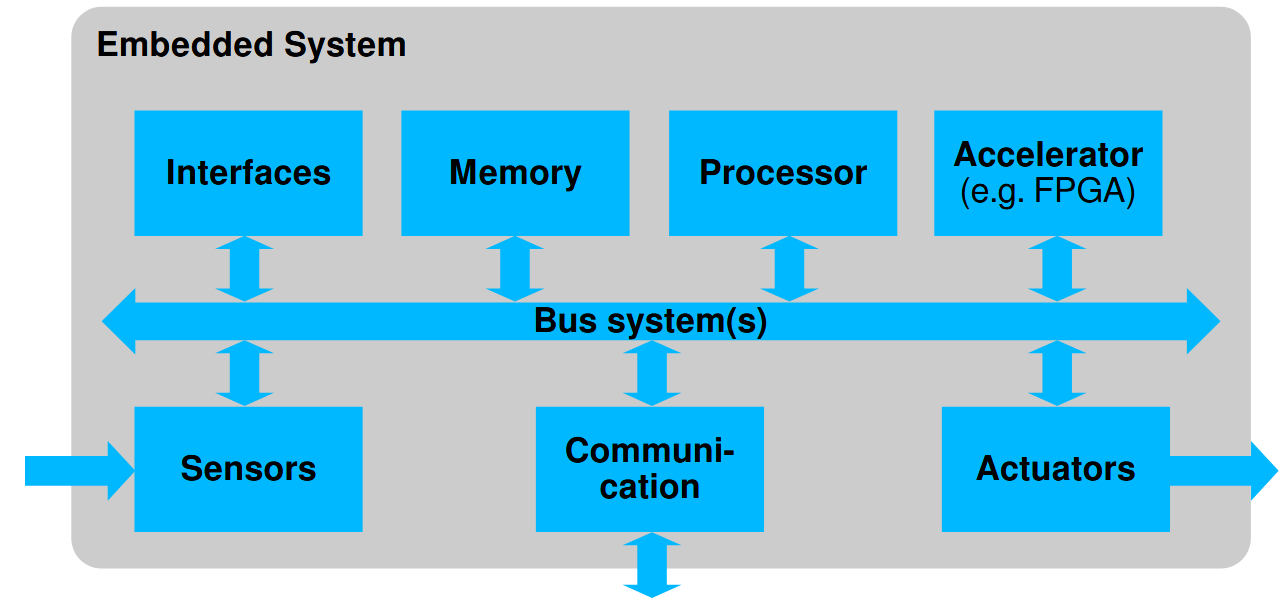
\includegraphics[width=.7\textwidth]{structure.png}
\end{figure}

\subsection{Power Consumption}
One of the most important constraints is power consumption! Minimising power consumption is important for the design of the power supply, the design of voltage regulators, dimensioning of interconnects, and short term cooling. Additionally, energy is expensive, batteries have limited capacity, and many other reasons.\\

Typical low-power design techniques include: (1) Low-power transistors (less speed), (2) dynamic power management (e.g. sleep modes), (3) dynamic voltage or frequency scaling.

\subsection{Quality}
Several aspects of quality must be taken into account when optimising cost:
\begin{itemize}
    \item \b{Defect Level (DL):} Fraction of defective parts delivered to customer (measured in DPM)
    \item \b{Yield:} Fraction of defect-free parts
    \item \b{Reliability:} Probability that a part will work correctly during its lifetime (safety-critical)
\end{itemize}

\subsection{Pareto-Frontier}
Pareto-Frontier analysis can be used for multiple target optimization by quantifying the design targets (as parameter vectors):\\[0.5em]
Given two solutions \f{A=(a_1, ..., a_m)} and \f{B=(b_1, ..., b_m)}, then \f{A} is dominating/pareto-superior to \f{B} iff \f{\forall j: a_j\geq b_j \wedge \exists i: a_i > b_i}. 


\section{Memory}
% Locality, memory hierarchies, cache systems, scratch pad memory, general types
Nowadays there are two types of machine models: more flexible "von Neumann" machines (which use one homogeneous memory for instructions and data), and more secure "harvard" machines which separate instruction and data memory.\\

One of the biggest issues in modern computing is the "memory wall", which is a synonym for the fact that processor speed is (increasingly) far faster than memory access times.

\subsection{Locality}
Programs tend to use data and instructions with addresses near or equal to those they have used recently. Recently referenced items are likely to be referenced again in the near future (temporal locality). Items with nearby addresses tend to be referenced close together in time (spatial locality).

\subsection{Memory Hierarchy}
For efficiency, fast memory access times and large memory sizes are required. However, not all memory is required all the time. This results in a trade-off problem: Latency vs cost + energy.\\
\begin{figure}[h!]
    \centering
    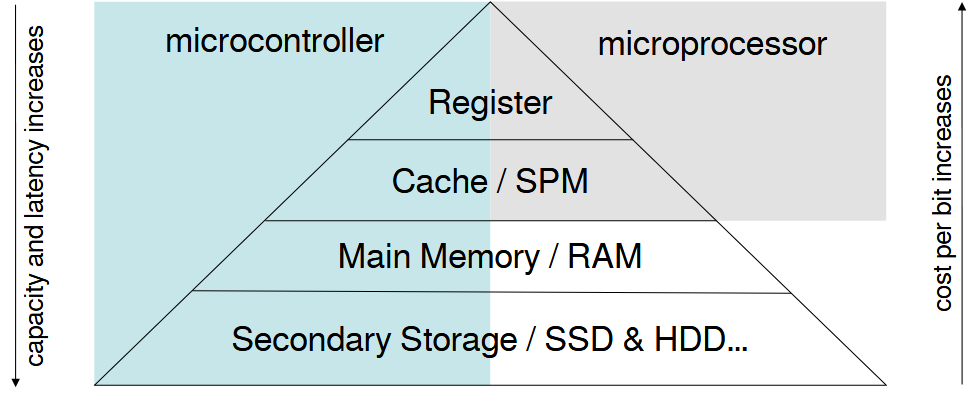
\includegraphics[width=.7\textwidth]{memory1.png}
\end{figure}

\subsection{Cache} Smaller, faster torage that acts as staging area for subset of data in a larger, slower device. Data is copied in block-sized units from main memory. Main question is which cache blocks to map the memory blocks to?\\[0.5em]
\b{Direct Mapping:} [Cache block address] = [Memory block address] mod [\# cache blocks]\\[0.5em]
\b{Associative Cache:} k blocks are in cache associated with same index. Cache tags are used to link to a specific set of memory blocks by comparing tags. When cache is full, replace block using FIFO or LRU (least recently used).\\

\b{Note:} For the Worst Case Execution Time analysis one has to assume that (almost) every access to the cache results in a cache miss.

\subsection{Memory Types}
\b{Non-volatile:} Keeps memory state without power (e.g. Flash, EPROM), read-only, usually slow and limited in number of write cycles, stores programs and rarely data.\\[0.5em]
\b{Volatile:} Keeps state only for short time, SRAM for fast and deterministic access (but power hungry, used as Cache), DRAM which depends on access order and needs periodic refresh

\subsection{\ac{spm}}
\acp{spm} are small physical memories directly mapped into the CPU's address space. This makes them fast and predictable and less power intensive. Usually frequently used instructions, variables, and intermediate results are stored in the SPM. SPM does not use tags, memory is directly accessed by the address.

\newpage
\section{Buses and Communication}
\subsection{I/O Access}
\b{Memory-mapped I/O:} The components get mapped into the controller address space, enabling convenient transfers as writing to the memory address sends data to the component. Downside: May keep CPU busy and needs polling for updates.\\

\b{Port-mapped I/O:} Uses special CPU instruction to transfer bytes. Data moves from one component via a bus address to the memory address. Also keeps CPU busy and needs polling for updates.

\subsection{\ac{dma}}
\ac{dma} is the component used in most \f{\mu C}, it offloads I/O transfers from the CPU.
\begin{enumerate}
    \item CPU instructs it to copy n bytes from the I/O device to a known location in the memory \b{directly}.
    \item DMA signals the CPU when the transfer is complete. In the mean time, the CPU is free.
\end{enumerate}
\vspace*{1em}
The usage of DMA gives rise to the issue of \b{cache coherency}:
\begin{itemize}
    \item CPU accesses location X in memory, the current value will be stored in the cache
    \item Operations on X will update the cached copy of X, but not the external memory version
    \item If the cached copy of X is not invalidated when a device writes a new value to the memory, then the CPU will operate on a stale value of X
\end{itemize}
To mitigate this issue, e.g. simple 'invalidate' flags can be broadcasted onto the bus on every write.

\subsection{Interrupt Requests (IRQs)}
Interrupts trigger the CPU on events, e.g. when a DMA operation is finished, on a keyboard press, or on a timeout. The procedure works as follows:\\

(1) Interrupt request gets triggered \f{\ \rightarrow\ } (2) Stop current execution of program and save context \f{\ \rightarrow\ } (3) Execute interrupt handler \f{\ \rightarrow\ } (4) Once finished, reload context and continue.


\subsection{Pulse Width Modulation}
How can a \f{\mu C} communicate with other digital modules (sensors, actuators, display modules, ...)?\\
\f{\rightarrow\ } For sensor and actuators, Pulse Width Modulation (PWM) is among the most frequent methods.
\begin{itemize}
    \item PWM is a digital modulation method to represent a signal as a rectangular wave with varying duty cycle \f{D} (i.e. proportion of 'on' time over regular interval)
    \item PWM can control electrical signal power or amplitude, e.g. to switch power supply
    \item Low power loss: No current in 'off' signal state; no voltage drop over switch in 'on' state
\end{itemize}

\b{Triangle Waverforms:} Three types (lead, centre, trail), the name describes the location of the peak\\[.5em]
\b{Intersective PWM:} Simple PWM generator principle with fixed period \f{T} and varying duty cycle. Uses a comparator to switch PWM output state (high, low) when input wave intersects with triangle wave.

\subsection{Inter-Integrated Circuit (I\f{^2}C)}
I\f{^2}C is a single-ended, synchronous, multi-controller/multi-target ("master-slave") serial bus. It has two lines: SCL (clock) and SDA (data).
\begin{figure}[h]
    \centering
    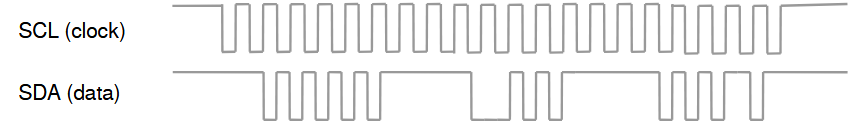
\includegraphics[width=.6\textwidth]{lines.png}
\end{figure}
\begin{figure}[h]
    \centering
    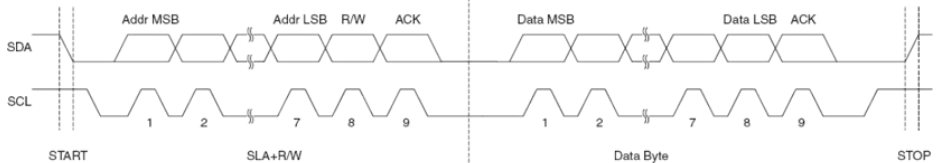
\includegraphics[width=.8\textwidth]{i2c.png}
\end{figure}

\subsection{Serial Peripheral Interface (SPI)}
SPI is a full-duplex, synchronous, master-slave, serial communication bus with 4 lines: SS/CS (chip/ slave select), SCLK (clock), MOSI/PICO (main data), and MISO/POCI (sub data).\\
While I\f{^2}C has a max bandwidth of 5Mbit/s, SPI has an arbitrary bandwidth (no max clock speed). Data is transferred in 4-16 bits.

\subsection{Testing and Debugging}
\subsubsection{Emulation}
Imitate behaviour of target system as close as required, thus substituting the object that is emulated. The internal state of the emulation mechanism does not have to accurately reflect the internal state of the target as long as the behaviour matches.

\subsubsection{Simulation}
Evaluate with a model of the target system. Ideally, the simulation makes properties of the target system observable. \b{A simulation does not always lead to emulation.}

\subsubsection{On-Target}
Evaluate (behaviour) on actual target hardware. The evaluation is usually done in a lab or simulation environment to control external influences.

\subsubsection{In-Field}
Evaluate on actual target hardware within the targeted application environment.

\subsubsection{JTAG}
A boundary scan bus for testing and debugging integrated circuits. It features a serial protocol with 5 lines: TDI (test data in), TDO (test data out), TCK (test clock), TMS (test mode select), and TRST (test reset, optional). Typically operates at 10-100MHz.\\
JTAG can be used for design verification and debugging (controllability), automated manufacturing tests, commissioning (programming of non-volatile memories), and to hack devices (all without physical access to every PCB line). For authentication it uses chain encryption.



\section{Sensors and Actuators}
\subsection{Measurements}
Sensors model a state of the environment through (time discrete) observations.\hfill
\begin{figure}[h]
    \centering
    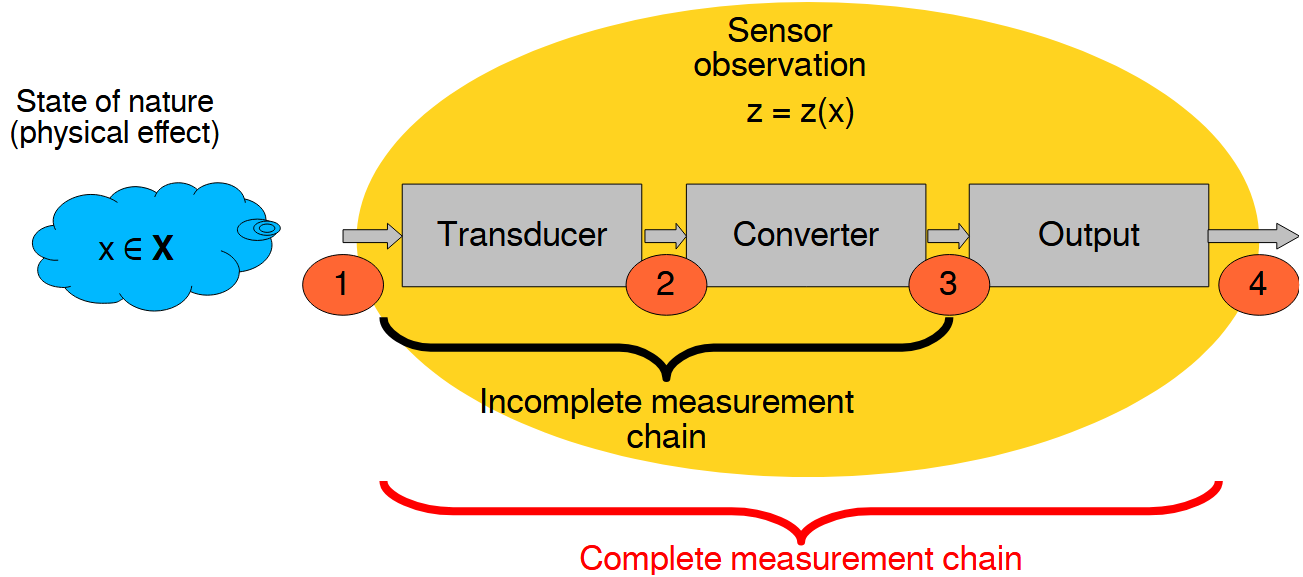
\includegraphics[width=.6\textwidth]{measure.png}
\end{figure}

The (analogue) signal captured by sensors is then digitised, i.e. converted from being continuous in \f{t,x} to being dicontinuous in both dimensions. To achieve this, different conversion strategies exist, all differing in conversion speed, accuracy of the values, and amplitude resolution after quantisation.\hfill
\begin{figure}[h!]
    \centering
    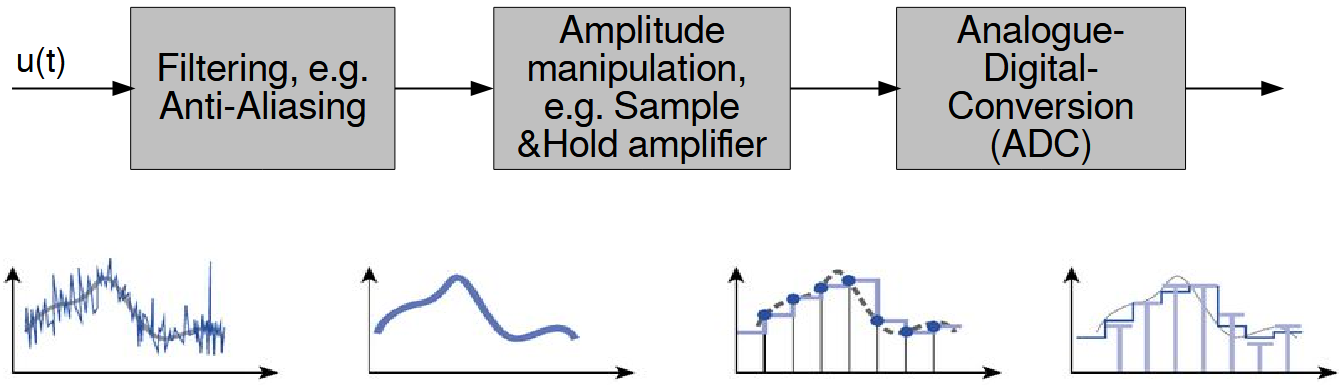
\includegraphics[width=.7\textwidth]{signals.png}
\end{figure}
% \noindent
\subsection{Parallel/Direct Conversion}
\begin{wrapfigure}{r}{.3\textwidth}
    % \centering
    % 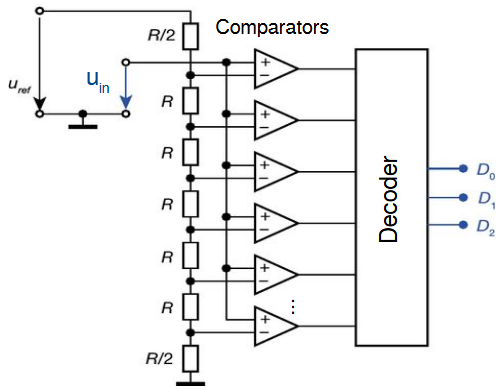
\includegraphics[width=.98\linewidth]{parallel.png}
    \raisebox{0pt}[\dimexpr\height-0.8\baselineskip\relax]{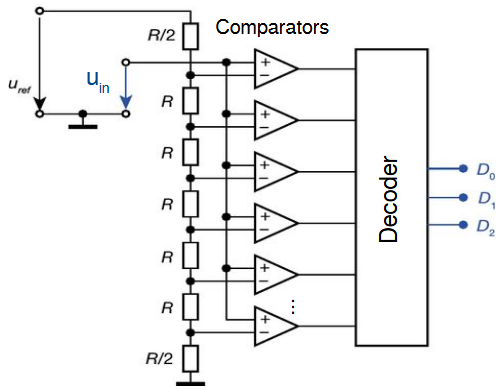
\includegraphics[width=.98\linewidth]{parallel.png}}
\end{wrapfigure}
Parallel converters work by comparing input voltage to a reference voltage using \f{2^n-1} parallel comparators.

The example on the right shows a 3-Bit converter. This approach is typically limited to \f{2^{N=8}=256} states and achieves frequencies greater than 1GHz.

To convert an n-bit digital signal into analogue, one can then use a parallel DAC as pictured below (n switches). The problem is that digital switches could be asynchronous, causing undefined u\f{_{\textrm{out}}}.
\vfill
\begin{figure}[h]
    \centering
    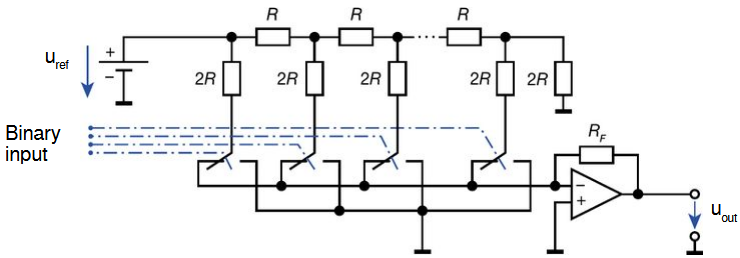
\includegraphics[width=.6\textwidth]{dac.png}
\end{figure}
\vfill
\clearpage

\subsection{Successive Approximation}
\begin{wrapfigure}{r}{.3\textwidth}
    % \centering
    % 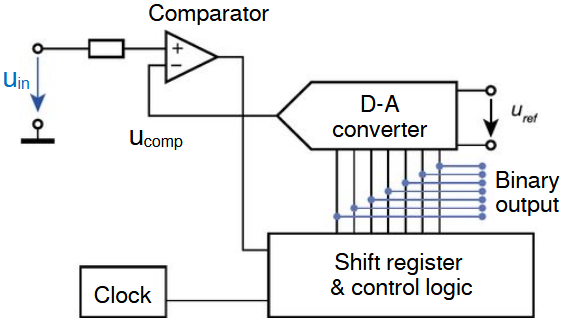
\includegraphics[width=.98\linewidth]{successive.png}
    \raisebox{0pt}[\dimexpr\height-2\baselineskip\relax]{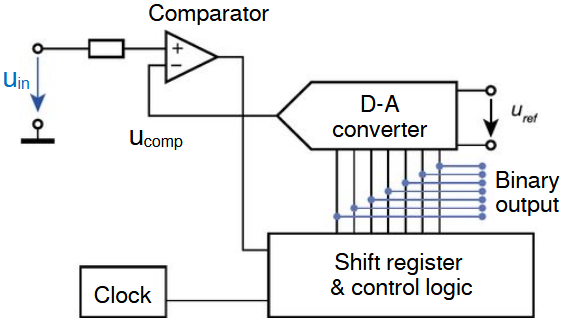
\includegraphics[width=.98\linewidth]{successive.png}}
\end{wrapfigure}
Successive Approximation is a sequential conversion technique that works according to the \b{weighting principle}. 

A DAC creates different reference voltages to be compared to the input. SA can resolve 24bits and upwards at a frequency of around 1MHz.

\subsection{Sample \& Hold}
The idea is to charge up to u\f{_{\textrm{in}}} as fast as possible (sample) and hold u\f{_{\textrm{out}}} constant for as long as possible.
\begin{figure}[h]
    \centering
    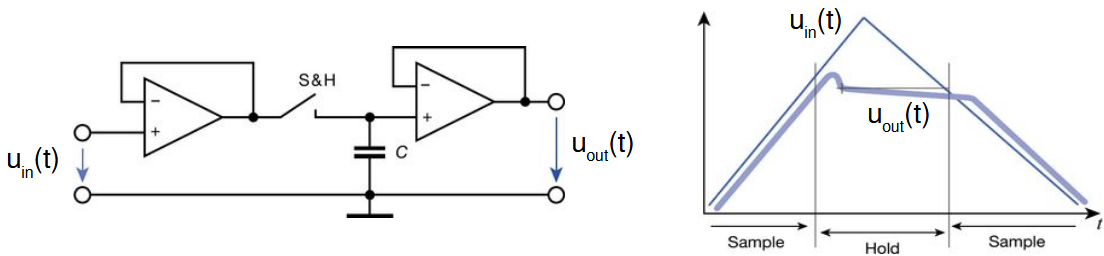
\includegraphics[width=.65\textwidth]{sh.png}
\end{figure}

\subsection{Dual/Multi-Slope Integrating Converter}
The main idea behind this technique is to convert and unknown voltage into a time delay, which is then encoded. It is accurate, produces low noise, has a linear transfer function, but is rather slow with a max. frequency of around 0.1-1kHz.
\begin{enumerate}
    \item Integrate u\f{_{\textrm{in}}} for fixed time (until counter flips to 0), results in u\f{_{\textrm{C}}}
    \item Apply u\f{_{\textrm{ref}}} with opposite polarity to integrator until 0V, thus comparator zeros and blocks clock at gate to maintain count result 
    \item Encode u\f{_{\textrm{in}}} as a function of u\f{_{\textrm{ref}}}, run-up time \f{t_0} and run-down time \f{t_U}
\end{enumerate}

\subsection{Aliasing}
Aliasing describes the effect when e.g. car wheels seem to spin backwards while accelerating. The same effect can also occure when sampling from an input signal.

To avoid aliasing, sampling intervals \f{T_s = 1/f_s} must be carefully chosen so that they can represent the original signal. A signal with maximum frequency of \f{f_{\textrm{in}}} must be sampled at \f{f_s\geq 2f_{\textrm{in}}}. Aliasing orrurs when \f{f_s < 2 f_{\textrm{in}} \leftrightarrow 0.5f_s < f_{\textrm{in}}}.

For a signal with two frequency components, one must sample at \f{f_s \geq 2(f_b - f_a)} to prevent aliasing.\hfill
\newline

More generally, given a sampling rate \f{f_s}, two frequencies \f{f} and \f{f'} are aliases of each other if \f{\exists k\in\mathbb{N}: f' = f + kf_s}. The \b{Nyquist Theorem} states, that the only range in which the original frequency can correctly be sampled/reconstructed is the \b{Nyquist bandwidth} from 0 to \f{0.5f_s}. 

Example: sampling at \f{0.2f_s \rightarrow f_s \geq 5f_{\textrm{in}}\rightarrow\textrm{ no aliasing}}.

\subsection{Aliasing Filters}
\b{Baseband sampling:} All signals of interest lie within Nyquist bandwidth (first Nyquist zone). Images at higher frequencies are filtered.\hfill\\[.5em]
\b{Undersampling:} Sampling signals outside first Nyquist zone. Image in first Nyquist zone contain all information in frequency-reversed order. Sampled signal may lie in any Nyquist zone. Image in first Nyquist zone retains all information. For this the Nyquist criterion is updated to \f{f_s\geq2\Delta f} where \f{\Delta f} is the bandwidth of the signal of interest.

\clearpage
\begin{figure}[t]
    \centering
    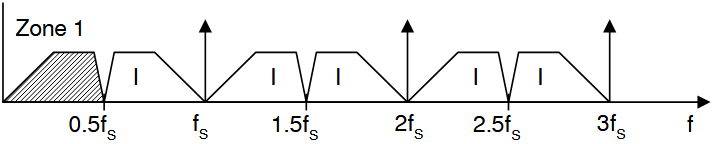
\includegraphics[width=.5\textwidth]{nyquist.png}
\end{figure}
\begin{figure}[t]
    \centering
    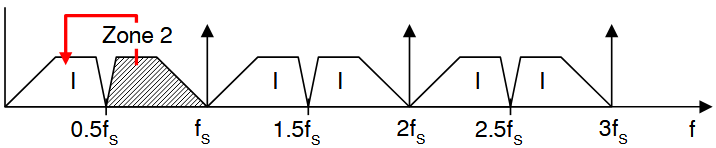
\includegraphics[width=.5\textwidth]{nyquist2.png}
\end{figure}






\section{Processors and Controllers}
\subsection{Microprocessor}
The microprocessor is \it{just} the computing unit and has to be complemented by different types of memory, I/O interfaces and other system components. They are usually fast but therefore expensive.

\subsection{Microcontroller}
A microcontroller (\f{\mu C}) is a System-on-Chip (SoC), which contains all basic components such as memory, timers, and various I/O interfaces (I\f{^2}C, SPI, UART). In comparison to microprocessors they are slower, but also cheaper and more energy efficient.

Classically they are used, when control operations are more frequent than data intensive computing (e.g. in multimedia).
\newline

To use a \f{\mu C}, the ES needs to fulfill multiple efficiency requirements: Energy efficiency (especially when using batteries), memory efficiency (thus code and architecture efficiency), run-time efficiency (processing efficiency for real-time use critical)
\section{Embedded AI}
End devices at the end of a network are called edge devices. Running AI (EAI) directly on these devices can have some advantages, but is usually much more complex and requires adjustments for individual devices.\hfill\\

\b{Advantages:} Maximise real-time performance (inference), privavy, reduce bandwidth requirements, cost, no network delay, offline use\hfill\\[0.5em]
\b{Drawbacks:} Very limited compute power, training and deployment has to be taylored for device\hfill

\subsection{Distributed Training}
\b{Centralised (level 1-3):} Model is trained in the cloud, end devices collect data and send it to the cloud, the cloud returns the inference results (during inference)\\[0.5em]
\b{Decentralised (level 5):} Each device trains its own model locally (with local data), to obtain global model all devices need to share model updates via network, ideal for privacy\\[0.5em]
\b{Hybrid (level 4-5):} Combines centralised and decentralised approach (e.g. cloud can be used to additionally train on public data)

\clearpage
\subsection{Model Compression \& Optimisation}
Since memory and efficiency are hard requirements in ES, the used models often need to be adjusted to fit onto the device (either before training when training on the device itself, or before deployment when training in the cloud).

\subsubsection{11.2.1 Compression}
\b{Weight pruning:} Removes redundant model weights (after training), requires post-finetuning to minimize accuracy reduction \\[0.5em]
\b{Data quantisation:} Replace number representation with lower-memory representation (e.g. 32-bit float to 16-bit float), reduces memory usage and accelerates computation

\subsubsection{11.2.2 Optimisation}
\b{Model partitioning:} Partition the model and distribute partitions between device and cloud; can be used to optimise latency, energy, and privacy\\[0.5em]
\b{Early exit:} Leverage output data of early layers (inference using partial model)\\[0.5em]
\b{Edge caching:}  Optimises latency by caching latest model inference results at network edge\\[0.5em]
\b{Model selection:} Dynamically select DNN model from a set during inference\\[0.5em]














% \input{chapters/12_vhdl.tex}


\end{document}